%
% File eamt20.tex
%
% Contact: cettolo@fbk.eu, mlf@dlsi.ua.es

%%% To ease future customizations, various replaceables have been paramaterized
%%% as listed in the newcommands section

\documentclass[11pt]{article}
\usepackage{eamt20}
\usepackage{times}
\usepackage{url}
\usepackage{latexsym}
\usepackage[small,bf]{caption} % added MLF 20171211
\setlength\titlebox{6.5cm}    % Expanding the titlebox
%%% YOUR PACKAGES BELOW THIS LINE %%%


\newcommand{\confname}{EAMT 2020}
\newcommand{\website}{https://eamt2020.inesc-id.pt}
\newcommand{\urlwebsite}{https://eamt2020.inesc-id.pt}
\newcommand{\contactname}{the general chair, Mikel L.\ Forcada}
\newcommand{\contactemail}{\texttt{mlf@ua.es}}
\newcommand{\conffilename}{eamt20}
\newcommand{\downloadsite}{https://eamt2020.inesc-id.pt\#templates}
\newcommand{\paperlength}{$10$ (ten)}
\newcommand{\shortpaperlength}{$10$ (ten)}
\newcommand{\projectlength}{$2$ (two)}
\newcommand{\translatorlength}{$10$ (ten)}

\title{Instructions for \confname\ Proceedings}

\author{First Author\\
  Affiliation / Address line 1\\
  Affiliation / Address line 2\\
  Affiliation / Address line 3\\
  {\tt email@domain}  \And
  Second Author\\
  Affiliation / Address line 1\\
  Affiliation / Address line 2\\
  Affiliation / Address line 3\\
  {\tt email@domain}}

\date{}

\begin{document}
\maketitle
\begin{abstract}
  This document contains the instructions for preparing a camera-ready
  manuscript for the papers in the
  proceedings of \confname . The document itself
  conforms to its own specifications, and is therefore an example of
  what your manuscript should look like. Authors are asked to conform
  to all the directions reported in this document.
\end{abstract}

\section{Credits}

This document is derived from the instructions for EAMT 2018 % update this list at next change
which was the latest in a long line of adaptations: EAMT 2009, EAMT 2011, EAMT 2012, EAMT 2014, EAMT 2015, EAMT 2016, EAMT 2017, Coling 2008, ACL-07, Coling/ACL-06, EACL-06, ACL-05 and EACL-03.  All these were based on the formats of earlier ACL and EACL Conference proceedings.  Those versions were written by several people, including John
Chen, Henry S. Thompson and Donald Walker.

\section{Introduction}

The following formatting instructions are directed to authors of
papers accepted for publication in \confname{} proceedings.

See also the
conference website\footnote{\urlwebsite} for additional
advice and information regarding submission.  All authors are required to adhere to these
specifications. Authors are required to submit their papers in PDF  (Portable Document
Format). The proceedings will be printed on
{\bf A4 paper}. Authors from countries in which access to
word processing systems is limited should contact \contactname~at \contactemail~ as soon as possible.

\section{General Instructions}

Manuscripts must be in two-column format.  Exceptions to the
two-column format include the {\nobreak{title}}, authors' names and complete
addresses, which must be centered at the top of the first page, and
any full-width figures or tables (see the guidelines in
Subsection~\ref{ssec:first}). {\bf Type single-spaced.}  Start all
pages directly under the top margin. See the guidelines later
regarding formatting the first page.

See Section~\ref{sec:length} for information on the
maximum number of pages.

If you are using Overleaf, you can use this document as a template for your submission. Simply create your own copy 
of this read-only document by clicking on the main Overleaf menu (see Figure~\ref{fig:clone})  at the top left of the document editing window and then click on ``Copy Project''. 
You can then modify the newly created document.

\begin{figure*}
 \centering
 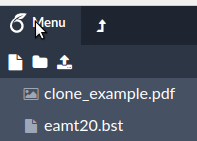
\includegraphics[scale=0.5]{clone1.png}
 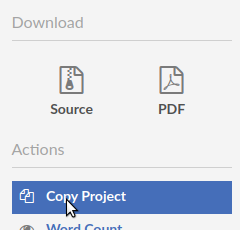
\includegraphics[scale=0.5]{clone2.png}   
 \caption{How to clone the LaTeX template in Overleaf}\label{fig:clone}
\end{figure*}

\subsection{Electronically-available resources}

This description is provided in \LaTeX2e (\nobreak{\conffilename.tex}) along
with the \LaTeX2e style file used to format it (\nobreak{\conffilename.sty})
and an EAMT bibliography style (\nobreak{\conffilename.bst}); and in PDF format
(\nobreak{\conffilename.pdf}). These files are all available at
\downloadsite. There is also a Microsoft Word
document template (\nobreak{\conffilename.dot}) available at the same URL. We
strongly re\-commend the use of these style files, which have been
appropriately tailored for the \confname~proceedings.


\subsection{Format of Electronic Manuscript}
\label{sect:pdf}

For the production of the electronic manuscript you must use Adobe's
Portable Document Format (PDF). This format can be generated from
postscript files. On Unix systems, you can use {\tt ps2pdf} for
this purpose. Under Microsoft Windows, you can use Adobe's Distiller
or GSview (File$>$Convert$>$pdfwrite); if you have \textit{cygwin}
installed, you can use \textit{ps2pdf}. Note that
some word processing programs generate PDF which may not include all
the necessary fonts (esp. tree diagrams, symbols). When you print or
create the PDF file, there is usually an option in your printer setup
to include none, all or just non-standard fonts.  Please make sure
that you select the option of including ALL the fonts. {\em Before
sending it, test your PDF by printing it from a computer different
from the one where it was created.} Moreover, some word processors may
generate very large postscript / PDF files, where each page is rendered
as an image. Such images may reproduce poorly. In this case, try
alternative ways to obtain the postscript and / or PDF. One way on some
systems is to install a driver for a postscript printer, send your
document to the printer specifying ``Output to a file'', then convert
the file to PDF.

% US Letter
%It is of utmost importance to specify the \textbf{US Letter format} (21.6 cm x
%27.9 cm) / (8.5 in x 11 in) when formatting the paper. When working with {\tt
%dvips}, for instance, one should specify {\tt -t letter}.

% A4
It is of utmost importance to specify the \textbf{A4 format} (21.0 cm
x 29.7 cm) / (8.3 in x 11.7 in) when formatting the paper. When working with
{\tt dvips}, for instance, one should specify {\tt -t a4}.

Print-outs of the PDF file on A4 paper should look like the present document,
which conforms to the formatting requirements. {\em Note that in order for
your paper to print correctly, you should disable centering and scale-to-fit
options on your printer.} If you cannot meet the above requirements about the
production of your camera-ready paper, please contact the programme chairs
as soon as possible.


\subsection{Layout}
\label{ssec:layout}

Format manuscripts two columns to a page, in the manner these
instructions are formatted. The exact dimensions for a page on
A4 paper are:

% US letter
% \begin{itemize}
% \item Left and right margins: 2.5 cm (1 in)
% \item Top margin: 2.5 cm (1 in)
% \item Bottom margin: 2.5 cm (1 in)
% \item Column width: 8 cm (3.15 in)
% \item Column height: 22.9 cm (9 in)
% \item Gap between columns: 0.5 cm (0.2 in)
% \end{itemize}

% A4
\begin{itemize}
\itemsep 0mm
\item Left and right margins: 2.5 cm (1 in)
\item Top margin: 2.5 cm (1 in)
\item Bottom margin: 2.5 cm (1 in)
\item Column width: 7.7 cm (3.1 in)
\item Column height: 23.7 cm (9.4 in)
\item Gap between columns: 0.5 cm (0.2 in)
\end{itemize}


\subsection{Fonts}

For uniformity, Adobe's {\bf Times Roman} font should be
used. In \LaTeX2e{} this is accomplished by putting

\begin{quote}
\begin{verbatim}
\usepackage{times}
\usepackage{latexsym}
\end{verbatim}
\end{quote}
in the preamble. If Times Roman is unavailable, use {\bf Computer
  Modern Roman} (\LaTeX2e{}'s default).  Note that the latter is about
  10\% less dense than Adobe's Times Roman font.


\subsection{The First Page}
\label{ssec:first}

Center the title, authors' names and affiliations across both
columns. Do not use footnotes for affiliations. Do not include the
paper ID number assigned during the submission process. Use the
two-column format only when you begin the abstract.

\paragraph{Title:} Place the title centered at the top of the first page, in
a 15-point bold font. Long titles should be typed on two lines without
a blank line intervening. Approximately, put the title at 2.5 cm (1 in) from
the top of the page, followed by a blank line, then the authors'
names, and the affiliations on the following line. Do not use only
initials for given names (middle initials are allowed). Avoid
capitalizing last names. The affiliation should contain the author's
complete address, and if possible an electronic mail address. Leave
about 2 cm (0.75 in) between the affiliation and the body of the first page.

\paragraph{Abstract:} Type the abstract at the beginning of the first
column. The width of the abstract text should be smaller than the
width of the columns for the text in the body of the paper by about
0.6 cm (0.25 in) on each side. Center the word {\bf Abstract} in a 12 point bold
font above the body of the abstract. The abstract should be a concise
summary of the general thesis and conclusions of the paper. It should
be no longer than 200 words.

\paragraph{Text:} Begin typing the main body of the text immediately after the
abstract, observing the two-column format as shown in the present document.
Use 11 point font for text. {\bf Indent} when starting a new paragraph, except
for the first paragraph following each heading.


\subsection{Sections}

\paragraph{Headings:} Type and label section and subsection headings in the
style shown on the present document.  Use numbered sections (Arabic
numerals) in order to facilitate cross references. Number subsections
with the section number and the subsection number separated by a dot,
in Arabic numerals. Do not number subsubsections. Use 11 point font for
subsection headings and 12 point font for section headings.

\paragraph{Citations:} Citations within the text appear in parentheses
as~\cite{Gusfield:97} or, if the author's name appears in the text itself, as
Gusfield~\shortcite{Gusfield:97}. Citations in parentheses should not be used
as linguistic phrases; for example, instead of ``\cite{Gusfield:97} \nobreak{argues}
that \ldots'' say ``Gusfield~\shortcite{Gusfield:97} \nobreak{argues} that \ldots''.
Treat double authors as in~\cite{Aho:72}, but write as in~\cite{Chandra:81} when more than
two authors are involved. 
\nobreak{Append} lowercase letters to the year in cases of ambiguity as in \cite{Gledson:08homog}. 
Collapse multiple citations in parenthesis as
in~\cite{Gusfield:97,Aho:72} and like this for multiple citations with the same-named \nobreak{author:}
% \cite{Tam:06,Tam:07,Gledson:08homog,Gledson:08websearch}
(Tam and Schultz, 2006, 2007; Gledson and Keane, 2008a,b).

\paragraph{References:} Gather the full set of references together under the
heading {\bf References}; place the section before any Appendices, unless they
contain references. Arrange the references alphabetically by the first
author's last-name, rather than by order of occurrence in the text, and invert
the first-name and last-name of the first author (only). Provide as complete
a citation as possible, using a consistent format, such as the one for {\em
Computational Linguistics\/} or the one in the {\em Publication Manual of the
American Psychological Association\/}~\cite{APA:83}.  Use of full names for
authors rather than initials is preferred.  Use full names for journals and
conferences, not abbreviations (for example ``45th Meeting of the Association
for Computational Linguistics'', not ``ACL07'').

The \LaTeX2e{} and Bib\TeX{} style files provided roughly fit the
American Psychological Association format, allowing regular citations,
short citations and multiple citations as described above.

\paragraph{Appendices:} Appendices, if any, directly follow the text and the
references (but see above).  Letter them in sequence and provide an
informative title: {\bf Appendix A. Title of Appendix}.

\paragraph{Acknowledgements:} the acknowledgement section should go as a last section immediately
\textit{before the references}.  Do not number the acknowledgement section.

\subsection{Footnotes}

Put footnotes at the bottom of the page and use
9-point font. They may be numbered or referred to by asterisks or
other symbols.\footnote{This is how a footnote should appear. Footnote numbers in the main text should follow punctuation}
Footnotes should be separated from the main text by a
line.\footnote{Note the line separating the footnotes from the text.}

\subsection{Other formatting hints}
Camera-ready papers should follow commonly accepted typographical conventions. Here are some of them:
\begin{itemize}
\item Use an en-dash (\LaTeX{} ``--'') for language pairs: ``English--Swahili'', not ``English-Swahili''.
\item Use an en-dash (\LaTeX{} ``--'') for number ranges: ``3--4'', not ``3-4''.
\item When typesetting math, function or variable names with more than one letter should be typeset in Roman (using \verb|\mathrm|), not italics: ``\(\mathrm{distance}(a,b)\)'', not ``\(distance(a,b)\)''.
\item When typesetting subscripts which are words or word abbreviations, make sure you typeset them in Roman (using \verb|\mathrm|): ``\(A_\mathrm{max}\)'', not ``\(A_\mathrm{max}\)''
\item Avoid informal abbreviations such as ``10k'' for ``10,000'' or ``4M'' for ``4,000,000'' or ``4 million''.
\item Separate quantities from units: ``4~GB'', not ``4GB''. Use an unbreakable space (\LaTeX{} ``\verb|~|'')
\end{itemize}

\subsection{Copyright}

\confname{} requires a copyright license statement. This should be inserted as
an unnumbered footnote on the first column of the first page. The \LaTeX{} style file
(and the Word template) adds the copyright statement automatically. Refer to the style file for instructions to
change this if required.

\subsection{Graphics}

\paragraph{Illustrations:} Place figures, tables, and photo\-graphs in the
paper near where they are first discussed, rather than at the end, if
possible.  Wide illustrations may run across both columns. Do not use
colour illustrations as they may reproduce poorly.

\paragraph{Captions:} Provide a caption for every illustration; number
each one sequentially in the form:  ``Figure 1. Caption of the
Figure.'', ``Table 1. Caption of the Table.''  Type the captions of
the figures and tables below the body, using 11-point text.


\section{Length of Submission}
\label{sec:length}

Unless otherwise specified, the maximum length is \paperlength~pages for research papers, \shortpaperlength~pages for user papers, \projectlength~pages for projects/products and
\translatorlength~pages for the translators' track papers. 
The page limit should be
observed strictly. All illustrations, references, and appendices must be
accommodated within these page limits, following the formatting instructions
given in the present document.

% \bibliography{\confname}

\begin{thebibliography}{}

\bibitem[\protect\citename{Aho and Ullman}1972]{Aho:72}
Aho, Alfred~V. and Jeffrey~D. Ullman.
\newblock 1972.
\newblock {\em The Theory of Parsing, Translation and Compiling}, volume~1.
\newblock Prentice-{Hall}, Englewood Cliffs, NJ.

\bibitem[\protect\citename{{American Psychological Association}}1983]{APA:83}
{American Psychological Association}.
\newblock 1983.
\newblock {\em Publications Manual}.
\newblock American Psychological Association, Washington, DC.

\bibitem[\protect\citename{{Association for Computing Machinery}}1983]{ACM:83}
{Association for Computing Machinery}.
\newblock 1983.
\newblock {\em Computing Reviews}, 24(11):503--512.

\bibitem[\protect\citename{Chandra \bgroup et al.\egroup }1981]{Chandra:81}
Chandra, Ashok~K., Dexter~C. Kozen, and Larry~J. Stockmeyer.
\newblock 1981.
\newblock Alternation.
\newblock {\em Journal of the Asso\-ciation for Computing Machinery},
  28(1):114--133.

\bibitem[\protect\citename{Gledson and Keane}2008a]{Gledson:08homog}
Gledson, Anne, and John Keane. 
\newblock 2008a. 
\newblock Measuring Topic Homogeneity and its Application to Dictionary-Based Word-Sense Disambiguation. 
\newblock {\em Coling 2008, 22nd International Conference on Computational Linguistics}, Manchester, UK.
\newblock 273--280.
\bibitem[\protect\citename{Gledson and Keane}2008b]{Gledson:08websearch}
Gledson, Anne, and John Keane. 
\newblock 2008b. 
\newblock Using Web-Search Results to Measure Word-group Similarity. \newblock {\em Coling 2008, 22nd International Conference on Computational Linguistics}, Manchester, UK.
\newblock 281--288.
\bibitem[\protect\citename{Gusfield}1997]{Gusfield:97}
Gusfield, Dan.
\newblock 1997.
\newblock {\em Algorithms on Strings, Trees and Sequences}.
\newblock Cambridge University Press, Cambridge, UK.

\bibitem[\protect\citename{Tam and Schultz}2006]{Tam:06}
Tam, Yik-Cheung and Tanja Schultz.
\newblock 2006. 
\newblock Unsupervised Language Model Adaptation Using
  \nobreak{Latent} Semantic Marginals.
\newblock {\em Interspeech 2006 -- ICSLP, Ninth International Conference on Spoken Language Processing}, 
Pittsburgh, Pennsylvania, paper 1705-Thu1A2O.2. 

\bibitem[\protect\citename{Tam and Schultz}2007]{Tam:07}
Tam, Yik-Cheung and Tanja Schultz.
\newblock 2007.
\newblock Correlated \nobreak{Latent} Semantic Model for
  Unsupervised Language Model Adaptation.
\newblock {\em Proceedings of ICASSP 2007, International Conference on 
  Acoustics, Speech, and Signal Processing}, Honolulu, Hawaii, Vol. IV, 41--44.

\end{thebibliography}

\end{document}
